\subsection{Field-Evidence Follow-up on New Documents}
\label{sec:eval:receipt_followup}

The first receipt study suggests that visible schema violations miss many
field-selection errors. Base and diagnostic prompts return all 60 input
graphs unchanged. Of 239 reference fields, 190 match exactly. The 49
mismatches include 27 case, spacing, punctuation, or amount-format differences,
ten span-boundary differences, eight different source values, and four values
absent from the normalized source. These categories describe reference
mismatches; they separate formatting from other repair targets.

We develop the field-evidence index in
Section~\ref{sec:framework:field_evidence} on 20 new receipts, then freeze it
before testing 60 further receipts. The original 60, development 20, and test
60 documents have disjoint IDs and no identical normalized transcripts.
The sample is fixed with seed 20260923. Test labels are downloaded only after
all test predictions are stored. Every arm receives the same field
definitions, numbered source lines, input graph, and instructions. Simple
uses these inputs directly; Evidence Index adds field anchors; SHACL adds
validation context. All three share the whitespace-consistent filter.

Development F1 is 80.00\% for the extracted graphs,
82.50\% for Simple,
85.00\% for Evidence Index, and
80.00\% for SHACL. We retain one fixed index design
and all three arms for the test. The primary comparison, frozen with the code
and scoring rules, is Evidence Index minus Simple in document-mean triple F1.

\begin{table*}[t]
\centering
\caption{Frozen follow-up on 60 new receipts. All repair arms share field
 definitions and source lines. Gate uses consistent whitespace matching.
 Exact match is over annotated fields.}
\label{tab:receipt_followup}
\small
\begin{tabular}{lrrrr}
\toprule
Method & Triple F1 & Exact graph & Normalized F1 & Preservation \\
\midrule
Extracted input & 0.7833 & 0.3500 & 0.7958 & 1.0000 \\
Simple, raw & 0.7875 & 0.2833 & 0.8083 & 0.9250 \\
Simple, gate & 0.7875 & 0.2833 & 0.8083 & 0.9250 \\
Evidence Index, raw & 0.8333 & 0.4000 & 0.8625 & 0.9306 \\
Evidence Index, gate & 0.8351 & 0.4000 & 0.8643 & 0.9306 \\
SHACL context, raw & 0.7833 & 0.2833 & 0.8042 & 0.9347 \\
SHACL context, gate & 0.7833 & 0.2833 & 0.8042 & 0.9347 \\
\bottomrule
\end{tabular}
\end{table*}

On the new test, extracted graphs reach 78.33\% F1.
Simple, Evidence Index, and SHACL with filtering reach
78.75\%, 83.51\%, and 78.33\%, respectively
(Table~\ref{tab:receipt_followup}). Simple changes F1 by
$0.42$ points relative to the input
(95\% CI: $[-4.17, 5.00]$).
The primary Evidence Index--Simple difference is
$4.76$ points (95\% CI: $[2.50, 7.26]$;
two-sided paired randomization $p=0.0004$).
Exact graph match is 28.33\%, 40.00\%, and
28.33\% for the three repair arms.

Simple restores 16 of 52 initially non-exact field values and changes 15 initially exact values to non-exact values.
Evidence Index restores 26 of 52 initially non-exact field values and changes 14 initially exact values to non-exact values.
SHACL restores 13 of 52 initially non-exact field values and changes 13 initially exact values to non-exact values.
The index restores 11 punctuation-only
differences and 6 span-boundary differences.
Of its lost exact matches, 10 preserve the numeric amount
but change its display format.
A separate numeric check removes currency prefixes and thousands separators
from the total field. Its accuracy is
58/60 for the input,
59/60 for Simple,
59/60 for Evidence Index, and
58/60 for SHACL.
This check distinguishes a changed amount from a changed display format.

Filtering rejects 1 candidate occurrence;
0 rejected candidates match a reference value.
The rejected address joins source fragments into a span absent from the text.
Filtering changes Evidence Index F1 by
0.18 points
and leaves the other two arms unchanged.

The three arms change 31, 39, and
28 of the 60 input graphs.
Mean repair request times are 7.91,
7.88, and 8.11 seconds,
with 1784, 2153, and
3404 input tokens. The run contains
240 actual requests for 60 extraction and 180 repair outcomes.
Raw and gated scores share responses; request times include pacing and retries.

\begin{figure}[t]
\centering
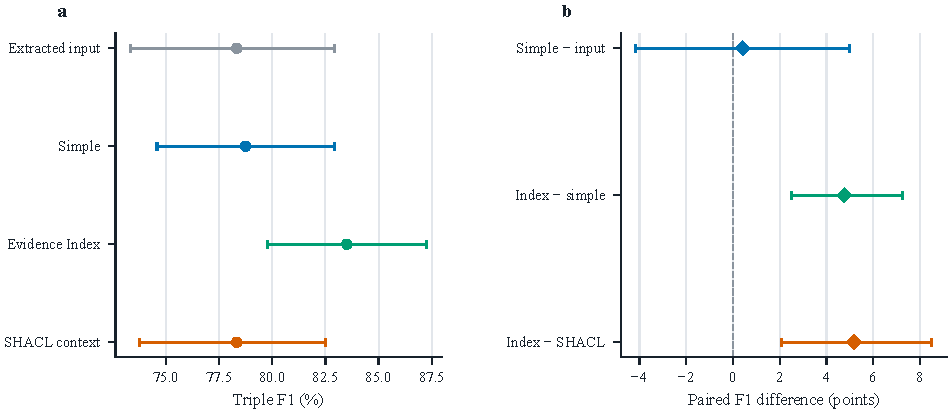
\includegraphics[width=0.98\textwidth]{figure/experiments/receipt_followup.pdf}
\caption{Follow-up on new receipts. Left: mean triple F1 with 95\% document-bootstrap
intervals. Right: paired F1 changes; intervals resample whole documents.
All repair methods share field definitions and source lines.}
\label{fig:receipt_followup}
\end{figure}
